\documentclass{article}

% Definitions
\newcommand{\pavo}{{\tt pavo}}  % you can use \pavo{} to print pavo as package
\newcommand{\code}[1]{{\tt #1}}  % way to plot out code
\setlength{\parindent}{0in}
\setlength{\parskip}{.1in}
\setlength{\textwidth}{140mm}
\setlength{\oddsidemargin}{10mm}
\usepackage{amsmath}
\usepackage{hyperref}

\usepackage{Sweave}
\begin{document}

\Sconcordance{concordance:pavo.tex:pavo.rnw:%
1 12 1 1 0 3 1 1 7 80 1 1 2 4 0 1 2 15 1}



\title{\pavo{}: {\bf P}erceptual {\bf A}nalysis, {\bf V}isualization and {\bf O}rganization of Color Data in R}
\author{Rafael Maia, Paul-Pierre Bitton, Chad Eliason}

\maketitle

\section*{Introduction}

\pavo{} is an R package developed with the goal of establishing a flexible and integrated 
workflow for working with spectral color data. It includes functions that take advantage of
new data classes in order to work seamlessly from importing raw data to visualization and 
analysis.

Although \pavo{} deals largely with spectral reflectance data from bird feathers, it is meant 
to be applicable for a range of taxa and applications. It provides flexible ways to input
spectral data from a variety of equipment manufacturers, process these data, extract variables 
and produce publication-quality graphics.

\pavo{} was written with the following workflow in mind:

% numbered list of things
\begin{enumerate}
\item {\bf Organize} spectral data by inputting files, processing spectra (e.g., to remove
noise, negative values, smooth curves, etc.)
\item {\bf Analyze} the resulting files, either using typical tristimulus color variables (hue,
saturation, brightness) or using visual models based on perceptual data from the taxon of 
interest.
\item {\bf Visualize} the output, with multiple options provided for exploratory analyses.
\end{enumerate}

Below we will show the main functions in the package in an example workflow. 

\section{Data Description}

The data used in this example is available from 
\href{https://github.com/rmaia/pavo/blob/master/vignette_data/vignette_data.zip}
{github by clicking here}. 
You can download and extract it to follow the vignette.

The data consists of reflectance spectra obtained using Avantes equipment and software from 
seven bird species: Northern Cardinal (\emph{Cardinalis cardinalis}), Wattled Jacana (\emph{Jaca
na jacana}), Baltimore Oriole (\emph{Icterus galbula}), Peach-fronted Parakeet (\emph{Aratinga 
aurea}), American Robin (\emph{Turdus migratorius}),  and Sayaca Tanager 
(\emph{Thraupis sayaca}). Several individuals were measured (sample size varies by species), and 
3 spectra were collected from each individual.

The samples do not have the same sample sizes and have additional peculiarities that should 
emphasize the flexibility \pavo{} offers, as we'll see below.

\section{Organizing and Processing Spectral Data}

\subsection{Importing Data}

The first thing we need to do is import the spectral data into R using the funciton 
\code{getspec()}. Since the spectra were obtained using Avantes software, we will need to 
specify that the files have the "\code{.ttt}" extension. Further, the data is organized in 
subdirectories for each species. \code{getspec} does recursive sampling, and may include the 
names of the subdirectories in the spectra name if desired. A final issue with the data is that 
it was collected using a computer with international numbering input, which means it uses commas 
instead of periods as a decimal separator. We can specify that in the function call.

I have downloaded the file and placed it in a directory called 
"\nolinkurl{/github/pavo/vignette_data}". By default, \code{getspec} will search for files in 
the default folder, but a different one can be specified:

\begin{Schunk}
\begin{Sinput}
> specs <- getspec("~/github/pavo/vignette_data/", ext="ttt", decimal=",", 
+                  subdir=T, subdir.names=F)
> specs[1:10,1:4]
\end{Sinput}
\begin{Soutput}
    wl cardinal.0001 cardinal.0002 cardinal.0003
1  300        5.7453        8.0612        8.0723
2  301        6.0181        8.3926        8.8669
3  302        5.9820        8.8280        9.0680
4  303        6.2916        8.7621        8.7877
5  304        6.6277        8.6819        9.3450
6  305        6.3347        9.6016        9.4834
7  306        6.3189        9.5712        9.3533
8  307        6.7951        9.4650        9.9492
9  308        7.0758        9.4677        9.8587
10 309        7.2126       10.6172       10.5396
\end{Soutput}
\begin{Sinput}
> dim(specs) #data has 214 spectra, from 300 to 700 nm
\end{Sinput}
\begin{Soutput}
[1] 401 214
\end{Soutput}
\end{Schunk}

When \pavo{} imports spectra, it creates an object of class \code{rspec}, which inherits attributes from the \code{data.frame} class:
\begin{Schunk}
\begin{Sinput}
> is.rspec(specs)
\end{Sinput}
\begin{Soutput}
[1] TRUE
\end{Soutput}
\end{Schunk}

If you already have multiple spectra in a single data frame that you'd like to use with \pavo{} 
functions, you can use the command \code{as.rspec} to convert it to an rspec object. The 
function will attempt to identify the wavelength variable or, if it doesn't have one, it can be 
specified in the function call.

\subsection{Processing Data}

\subsection{Averaging Spectra}

As previously described, our data constitutes of multiple individuals, and each was measured 
three times, as is common in order to avoid measurement bias. A good way to visualize the 
repeatability of our measurements is to plot the spectra of each individual separately. The 
function \code{explorespec} provides an easy way of doing so. You may specify the number of 
spectra to be plotted in the same panel using the argument \code{specreps}, and the function 
will adjust the number of panels per page accordingly. We will exemplify this function using 
only the 12 cardinal individuals measured:

\begin{Schunk}
\begin{Sinput}
> explorespec(specs[,1:37], specreps=3) 
> # 36 spectra plus the first (wl) column
\end{Sinput}
\end{Schunk}

\begin{figure} % h=here, t=top, b=bottom, p=floating page
\begin{center}
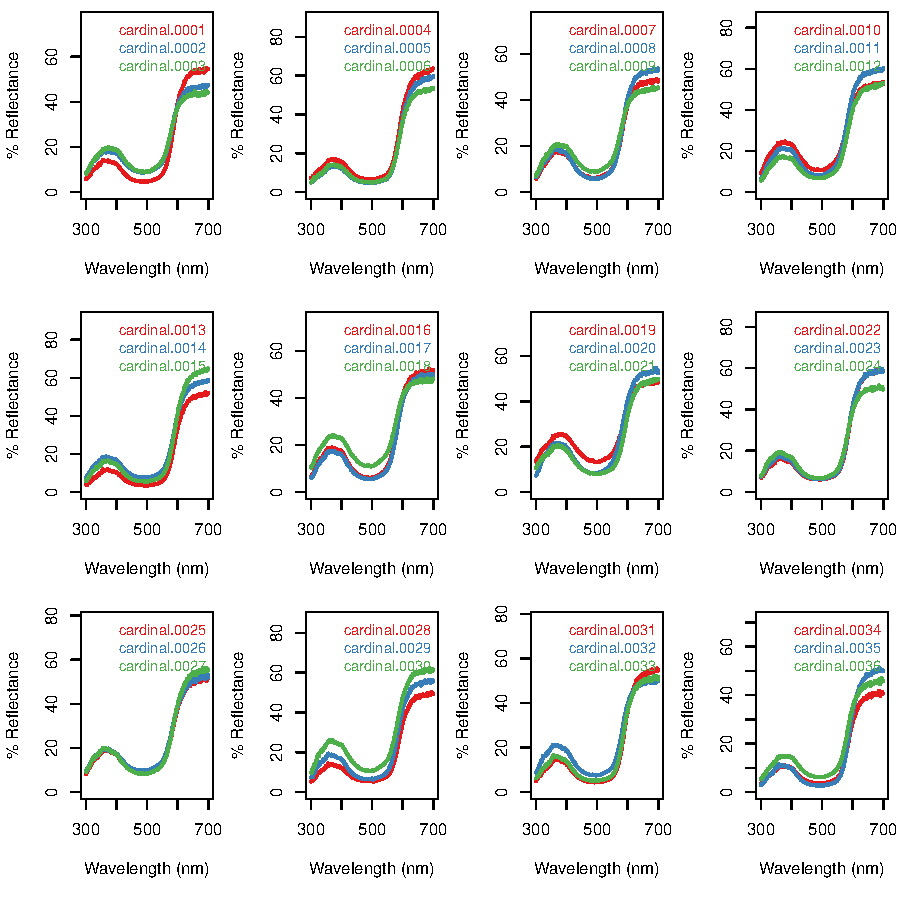
\includegraphics[width=5in]{pavo-explorespecfig}
\end{center}
\caption{Result from \code{explorespec}, showing the three measurements for each individual in separate panels}
\label{fig1}
\end{figure}

\clearpage{}

So our first step would be to take the average of each of these three measurements in order to 
obtain average individual spectra to be used in further analyses. The function \code{aggspec} 
does this. The \code{by} argument can be either a number (specifying how many specs should be 
averaged for each new sample) or a vector specifying the identities of the spectra to be 
combined (see below):

\begin{Schunk}
\begin{Sinput}
> mspecs <- aggspec(specs, by=3, FXN=mean)
> mspecs[1:5, 1:4]
\end{Sinput}
\begin{Soutput}
   wl cardinal.0001 cardinal.0004 cardinal.0007
1 300      7.292933      5.676700      6.387233
2 301      7.759200      5.806700      6.698200
3 302      7.959333      5.858467      6.910500
4 303      7.947133      6.130267      7.357567
5 304      8.218200      6.127933      7.195267
\end{Soutput}
\begin{Sinput}
> dim(mspecs) #data now has 72 spectra, one for each individual
\end{Sinput}
\begin{Soutput}
[1] 401  72
\end{Soutput}
\end{Schunk}

Now we'll use the \code{aggspec} function again, but this time to take the average spectrum for 
each species. However, each species has a different number of samples, so we can't use the 
\code{by} argument as before. Instead we will use regular expressions to create a species name 
vector by removing the numbers that identify individual spectra:

\begin{Schunk}
\begin{Sinput}
> # create a vector with species identity names
> spp <- gsub('\\.[0-9].*$','',names(mspecs))[-1]
> table(spp)
\end{Sinput}
\begin{Soutput}
spp
cardinal   jacana   oriole parakeet    robin  tanager 
      12        9        9       13       10       18 
\end{Soutput}
\end{Schunk}

Instead, we are going to use the \code{spp} vector we created to tell the \code{aggspec} 
function how to average the spectra in \code{mspec}:

\begin{Schunk}
\begin{Sinput}
> sppspec <- aggspec(mspecs, by=spp, FXN=mean)
> sppspec[1:5, ]
\end{Sinput}
\begin{Soutput}
   wl cardinal   jacana   oriole parakeet    robin
1 300 7.049397 7.334781 3.889693 7.629954 3.981747
2 301 7.254161 7.354033 3.905322 7.746882 3.914297
3 302 7.444275 7.452556 4.126619 7.886877 4.187073
4 303 7.820686 8.085541 4.390685 8.491367 4.507410
5 304 7.843394 7.714526 4.183637 8.658000 4.068800
    tanager
1  9.021043
2  9.525854
3  9.405980
4 10.199843
5  9.684522
\end{Soutput}
\begin{Sinput}
> explorespec(sppspec, 7)
\end{Sinput}
\end{Schunk}

\begin{figure}[h] % h=here, t=top, b=bottom, p=floating page
\begin{center}
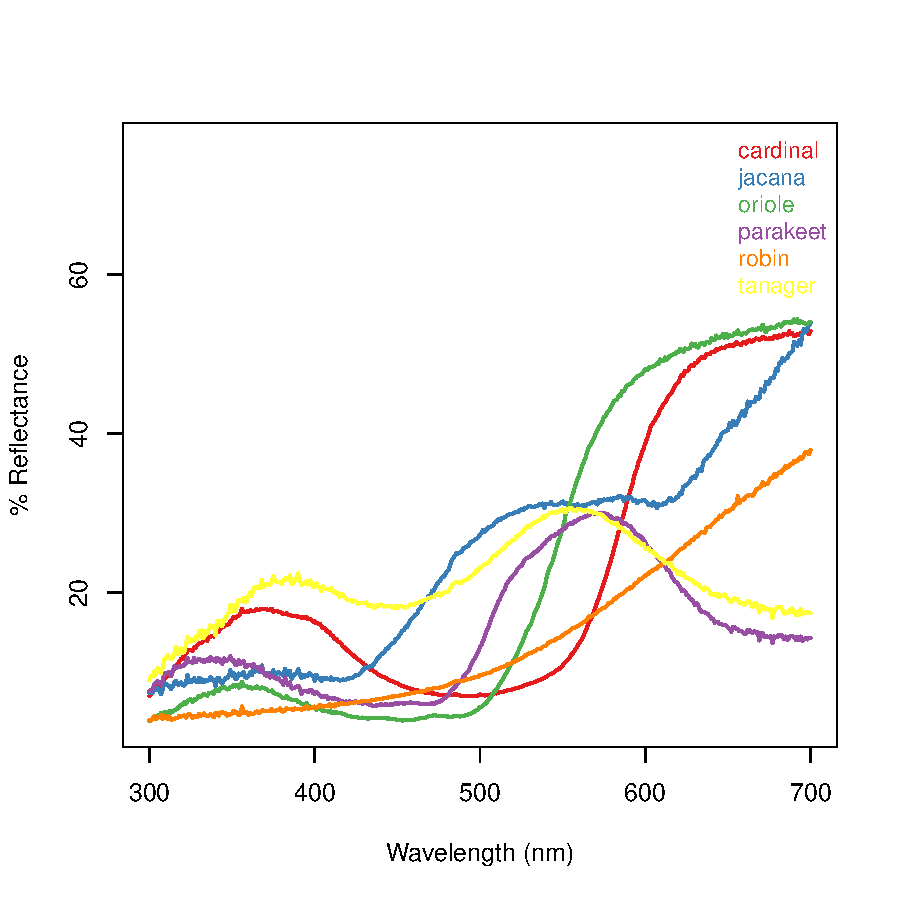
\includegraphics[width=4in]{pavo-exploresppmeans}
\end{center}
\caption{Result from \code{explorespec} for species means}
\label{fig2}
\end{figure}


\section{Visualizing Spectral Data}

\begin{Schunk}
\begin{Sinput}
> data(sicalis)
> par(mfrow=c(1,2))
> plot(sicalis, type='o', col=spec2rgb(sicalis))
> plot(procspec(sicalis, opt='smooth'), type='o', col=spec2rgb(sicalis))
\end{Sinput}
\begin{Soutput}
processing options applied:
 smoothing spectra with a span of 0.25 
\end{Soutput}
\begin{Sinput}
> 
> #plot(sicalis, type='s', col=spec2rgb(sicalis))
\end{Sinput}
\end{Schunk}



\begin{figure} % h=here, t=top, b=bottom, p=floating page
\begin{center}
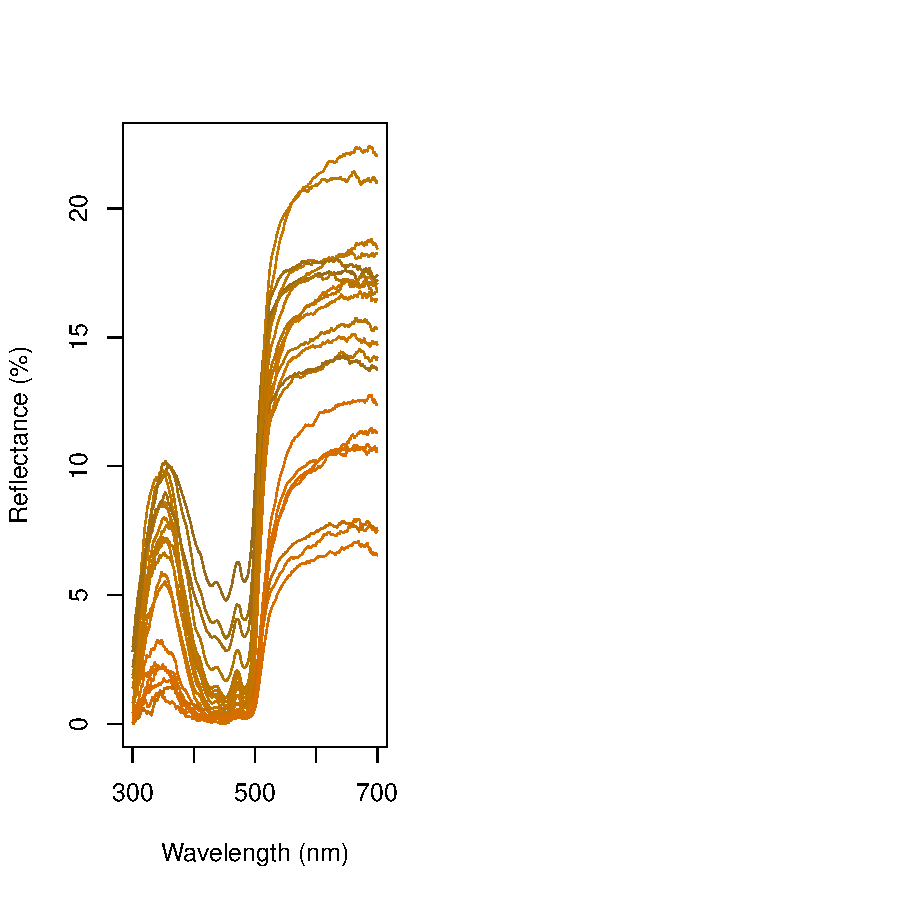
\includegraphics[width=4in, height=3in]{pavo-overlay}
\end{center}
\caption{Overlay plot with colors calculated from human color matching functions}
\label{figure:overlay}
\end{figure}

Colors can be mapped to spectra using \code{spec2rgb} as shown in 
Figure \ref{figure:overlay}.


\section{Analyzing Spectral Data}

\subsection{Overview}

\pavo{} offers two main approaches for spectral data analysis. First, variables can be 
calculated based on the shape of the reflectance spectra. By using special R classes for spectra 
data frame objects, this can easily be done using the \code{summary} function in an rspec 
object (see below). The second function for spectral shape analysis is \code{peakshape}, which returns descriptors for peaks in spectral curves, as outlined below.

Second, reflectance spectra can be analyzed accounting for the visual system receiving the color 
signal, therefore representing reflectance spectra as preceived colors. We have implemented 
Endler's (REF) segment analysis model, which approximates visual models but does not directly 
use sensory information; the model of Osorio \& Vorobyev (REF), which provides a flexible 
framework for visual modeling; and the tetrahedral color space (GOLDSMITH, ENDLER, STODDARD) 
which has been extensively developed to represent colors in the avian vision color space.

\subsection{Spectral Shape Analysis}

\textit{\textbf{Trichromatic variables}}

Obtaining trichromatic color variables (related to hue, saturation and value) is pretty
straightforward in \pavo{}. Since reflectance spectra is stored in an object of class 
\code{rspec}, the \code{summary} function recognizes the object as such and extracts 23 
variables, as outlined in MONTGOMERIE. Though outlined in a book chapter on bird coloration, 
these variables are broadly applicable to any reflectance data, particularly if the taxon of 
interest has color vision within the UV-human visible range.

The description and formulas for these variables can be found in Table \ref{table:tristim}.

\begin{Schunk}
\begin{Sinput}
> summary(sppspec)
\end{Sinput}
\begin{Soutput}
               B1       B2       B3      S1.UV  S1.violet
cardinal 8983.870 22.40367 52.96101 0.16618070 0.19132718
jacana   9668.442 24.11083 53.48957 0.09623268 0.11048401
oriole   9107.568 22.71214 54.31982 0.07474281 0.08314578
parakeet 6022.866 15.01962 28.82353 0.16803871 0.18515359
robin    5741.033 14.31679 37.96515 0.08500350 0.10012432
tanager  8516.756 21.23879 29.76561 0.20342675 0.23931496
            S1.blue  S1.green S1.yellow    S1.red        S2
cardinal 0.11784952 0.1900225 0.2517886 0.5332009  7.329535
jacana   0.19475522 0.3082406 0.2479744 0.4079294  6.883918
oriole   0.05721376 0.3256520 0.3630756 0.5491879 12.992914
parakeet 0.14334383 0.4252528 0.3397279 0.2717663  4.768352
robin    0.14429801 0.2675057 0.2668015 0.5099805  9.172749
tanager  0.26109724 0.3199401 0.2430633 0.2238215  3.120773
                S3         S4       S5       S6          S7
cardinal 0.3682957 0.15813546 4004.193 45.73531 -0.38403228
jacana   0.2469875 0.01690805 3312.697 45.71935 -0.46942827
oriole   0.3444943 0.06767440 5232.176 50.13910 -0.70982859
parakeet 0.4467452 0.23727515 1900.192 22.77878 -0.20889035
robin    0.3031191 0.01271259 2531.901 33.82625 -0.57712488
tanager  0.3341862 0.15240014 1105.252 20.22771 -0.08198454
                S8         S9        S10  H1  H2  H3
cardinal 2.0414210 -0.8373693  12.909318 700 425 596
jacana   1.8962165 -0.7357544 112.148743 700 388 504
oriole   2.2075903 -0.9257720  32.620756 700 388 500
parakeet 1.5166018 -0.5816948   6.391743 568 613 502
robin    2.3626975 -0.8148189 185.854859 700 349 500
tanager  0.9523946  0.0359801   6.249303 557 600 428
                 H4  H5
cardinal 1.54995089 617
jacana   0.85480076 463
oriole   1.15606660 538
parakeet 0.59271149 500
robin    1.15020735 637
tanager  0.04509807 512
\end{Soutput}
\end{Schunk}


% A table for filling in Montgomerie's color variables
\begin{table}[h]
\begin{center}
\begin{tabular}{l l l} \hline
{\bf Color} & \\
{\bf Variable} & {\bf Equation} & {\bf Description} \\ 
\hline
\code{B1} & {$\sum_{\lambda={300}}^{700} R_\lambda$} & \parbox[t]{3in}{Total brightness, total reflectance}  \\
\code{B2} & {$B_\text{1}/n_\text{wl}$} & \parbox[t]{3in}{Mean brightness.} \\
\code{B3} & {$R_\text{max}$} & \parbox[t]{3in}{Intensity.} \\
\code{S1} & {} & \parbox[t]{3in}{Chroma, spectral purity.} \\
\code{S2} & {$R_\text{max}/R_\text{min}$} & \parbox[t]{3in}{Spectral saturation} \\
\code{S3} & {} & \parbox[t]{3in}{} \\
\code{S4} & {} & \parbox[t]{3in}{} \\
\code{S5} & {} & \parbox[t]{3in}{} \\
\code{S6} & {} & \parbox[t]{3in}{} \\
\code{S7} & {} & \parbox[t]{3in}{} \\
\code{S8} & {} & \parbox[t]{3in}{} \\
\code{S9} & {} & \parbox[t]{3in}{} \\
\code{S10} & {} & \parbox[t]{3in}{} \\
\code{H1} & {$\lambda_\text{Rmax}$} & \parbox[t]{3in}{Hue: wavelength of peak reflectance} \\
\code{H2} & {} & \parbox[t]{3in}{} \\
\code{H3} & {} & \parbox[t]{3in}{} \\
\code{H4} & {} & \parbox[t]{3in}{} \\
\code{H5} & {} & \parbox[t]{3in}{} \\
\hline
\end{tabular}
\end{center}
\caption{\label{table:tristim}
The complete set of tristimulus variables calculated by \code{summary} in \pavo{}}
\end{table}

\clearpage{}

\textit{\textbf{Peak shape descriptors}}

Particularly in cases of reflectance spectra that have a single, discrete peak, it might be useful to obtain variables that describe that peak's properties. The \code{peakshape} function identifies the peak location (\code{H1}),  returns the reflectance at that point (\code{B3}), and identifies the wavelengths at which the reflectance is half that at the peak, calculating the wavelength bandwith of that interval (the \textbf{Full Width at Half Maximum}, or \code{FWHM}). The function also returns the half widths, which are useful when the peaks are located near the edge of the measurement limit and half maximum reflectance can only be reliably estimated from one of its sides.

If this all sounds too esoteric, fear not: \code{peakshape} has the option of returning plots indicating what it's calculating. The vertical continuous red line indicates the peak location, the horizontal continuous red line indicates the half-maximum reflectance, and the distance between the dashed lines is the FWHM:

\begin{Schunk}
\begin{Sinput}
> par(mfrow=c(2,3),mar = c(5, 4, 0.5, 0.5) + 0.1)
> peakshape(sppspec, plot=T)
\end{Sinput}
\begin{Soutput}
               B3  H1 FWHM HWHM.l HWHM.r status
cardinal 52.89508 687  104    100      4     OK
jacana   53.90258 700   NA     93     NA     OK
oriole   54.40384 692  148    141      7     OK
parakeet 30.05703 575  125     66     59     OK
robin    37.91676 700   NA    107     NA     OK
tanager  30.71021 555  232    142     90     OK
\end{Soutput}
\end{Schunk}

\begin{figure}[h] % h=here, t=top, b=bottom, p=floating page
\begin{center}
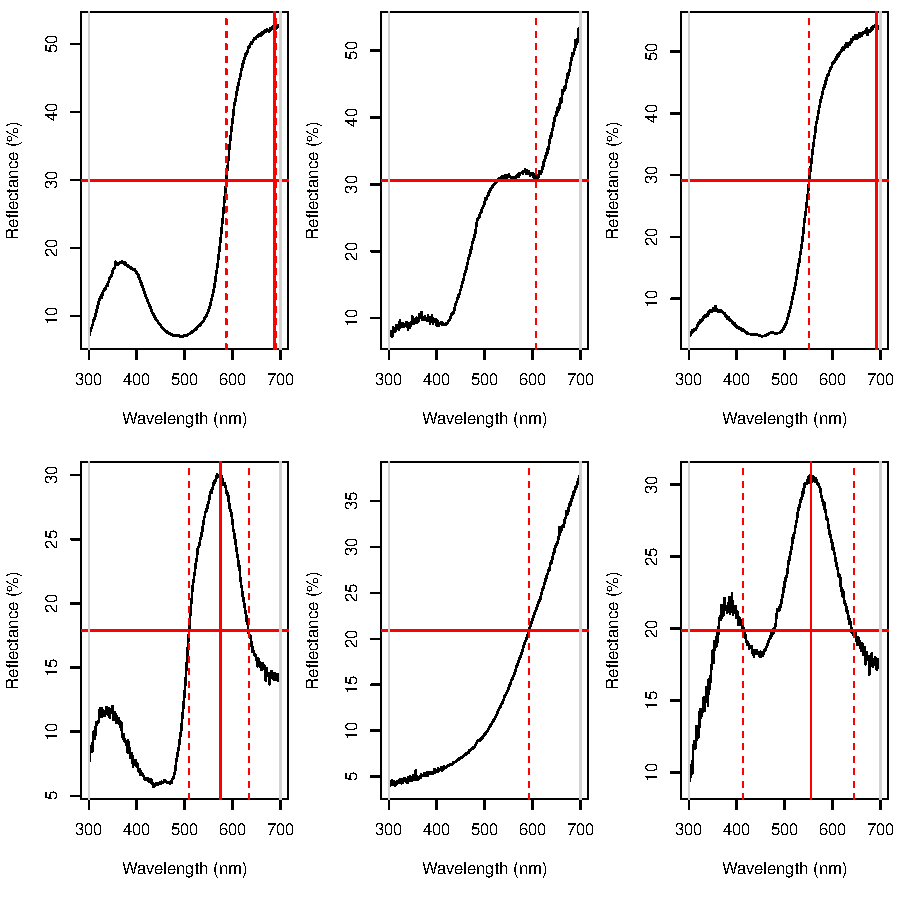
\includegraphics[width=6in, height=5in]{pavo-fwhm}
\end{center}
\caption{Plots from \code{peakshape}}
\label{figure:fwhm}
\end{figure}

\clearpage{}

As it can be seen, the variable is meaningless if the curve doesn't have a clear peak. Sometimes, such as in the case of the Cardinal (Figure \ref{figure:fwhm}, first panel), there might be a peak which is not the point of maximum reflectance of the entire spectral curve. The half-width can also be erroneously calculated when there are two peaks, as can be seen in the case of the Tanager (Figure \ref{figure:fwhm}, last panel). In this case, it's useful to set bounds when calculating the FWHM, using the \code{bounds} argument. \code{peakshape} also offers a \code{select} argument to facilitate subsetting the spectral data frame:

\begin{Schunk}
\begin{Sinput}
> peakshape(sppspec, select=2, bounds=c(300,500), plot=T)
\end{Sinput}
\begin{Soutput}
               B3  H1 FWHM HWHM.l HWHM.r status
cardinal 17.99853 369  100     47     53     OK
\end{Soutput}
\end{Schunk}

\begin{figure}[h] % h=here, t=top, b=bottom, p=floating page
\begin{center}
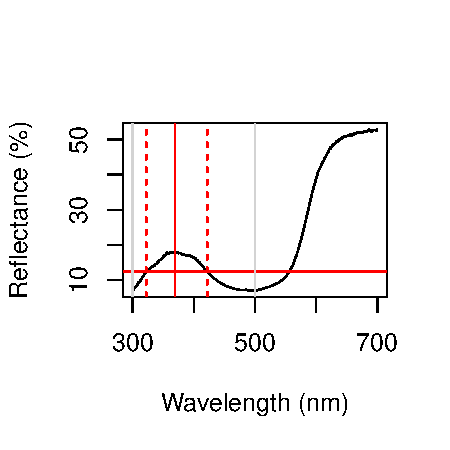
\includegraphics[width=3in, height=3in]{pavo-fwhm2}
\end{center}
\caption{Plot from \code{peakshape}, setting the bounds to 300-500nm}
\label{igure:fwhm2}
\end{figure}

\clearpage{}

\section*{Examples}


\begin{Schunk}
\begin{Sinput}
> hist(rnorm(50))
\end{Sinput}
\end{Schunk}


\subsection*{More examples}

Some more examples:

\bibliography{}

\end{document}
